\begin{abstract}
The exponential growth of connectivity and computing demand has made \gls{nfvi} major contributors to global energy consumption. Conventional network and service deployments, whether based on legacy hardware appliances or \gls{nfvi} stacks, struggle to dynamically provision resources for peak data traffic demand. This results in nearly constant energy consumption even during low-traffic periods, leading to inefficient resource use.
Network softwarization and virtualization have enabled flexible and programmable service deployments, which are beneficial for rapid and dynamic scaling of network functions. This paper validates energy-aware service and network orchestration with a \gls{zsm} framework for autonomous optimization of computing, network, and power resources from \gls{nfvi} on a use case focused on connected mobility, and in particular, smart traffic management. By modeling road traffic based on vehicle count and type and \gls{3gpp} profiles for data formats in vehicular communication scenarios, the \gls{zsm} framework adjusts services and resources to services requirements and to actual demand. Experimental validation on the real-life Smart Highway testbed in Antwerp (Belgium) demonstrates a strong correlation between vehicular traffic and power consumption, supporting the hypothesis that adaptive compute and network resource management reduces unnecessary energy use and advances the vision of sustainable and self optimizing \gls{6g} networks.
\end{abstract}
\glsresetall
\section{Energy-Awareness Experiment 1}\label{awar:1}
This is my starting point \cite{3gpp-ts-22-186,3gpp_ts_26_511_v18_1_0}

Every physical capability of the \gls{rsu} is different from each other in terms of maximum wattage.
When the \glspl{rsu} were stressed based on the amount of vehicles, they have a limit of watts also linked to the CPU consumption.

\begin{table}[htbp]
    \centering
    \caption{Average vehicular counts and power consumption per RSU.}
    \label{tab:rsu-traffic-power}
    \begin{tabular}{|c|cc|cc|}
        \hline
        \textbf{RSU} & \multicolumn{2}{c|}{\textbf{Night (17:00--06:00)}} & \multicolumn{2}{c|}{\textbf{Day (06:00--17:00)}}                        \\
        \cline{2-5}
                     & Vehicles                                           & Power (W)                                        & Vehicles & Power (W) \\
        \hline
        1            & 0                                                  & 59                                               & 4        & 58        \\
        2            & 1                                                  & 55                                               & 7        & 55        \\
        3            & 5                                                  & 56                                               & 23       & 56        \\
        5            & 2                                                  & 51                                               & 7        & 51        \\
        6            & 1                                                  & 60                                               & 5        & 60        \\
        7            & 6                                                  & 61                                               & 16       & 61        \\
        \hline
    \end{tabular}
\end{table}
\begin{table}[!t]
    \centering
    \caption{Location mapping between inductive sensors and \glspl{rsu} to monitor vehicular traffic per \gls{rsu} in the E13 Highway, Antwerp Belgium.}
    \label{tab:location-mapping-rsu}
    \begin{adjustbox}{max width=\columnwidth}
        \begin{tabular}{|l|c|l|l|}
            \hline
            \textbf{\gls{rsu}} & \textbf{Vehicles} & \textbf{RSU Location} & \textbf{Nearest Inductive Sensor} \\
            \hline
            1 & 12 & 51.210575, 4.46655        & 51.21056678, 4.466446158 \\
            3 & 25 & 51.215186667, 4.450568333 & 51.21587307, 4.452993707 \\
            7 & 12 & 51.210616667, 4.480896667 & 51.21066931, 4.480559376 \\
            8 & 26 & 51.211091667, 4.491425    & 51.21127494, 4.491424033 \\
            4 & 16 & 51.21574, 4.457151667     & 51.21577734, 4.457154961 \\
            6 & 16 & 51.211236667, 4.472586667 & 51.21121407, 4.472483657 \\
            \hline
        \end{tabular}
    \end{adjustbox}
\end{table}

Table~\ref{tab:rsu-max-capacity} summarizes the maximum number of users (U) and the corresponding maximum wattage (W) capacity for each \gls{rsu}. As shown, \gls{rsu} 5 supports the highest number of vehicles and reaches a higher power consumption compared to the others. This variation highlights the heterogeneous nature of the \glspl{rsu} in the testbed. Figure~\ref{fig:exp1-figure} visually presents the relationship between the number of vehicles and the power consumption for each \gls{rsu}, illustrating how the power usage increases with the load and reaches a plateau at the maximum capacity.

Max vehicles registered: 39 \gls{rsu} 5
\begin{table}[ht]
    \centering
    \caption{Maximum U and W capacity for each \gls{rsu}.}
    \begin{tabular}{ccc}
        \hline
        \gls{rsu} & Max U & Max W Capacity \\
        \hline
        1         & 27    & 69             \\
        2         & 27    & 67             \\
        3         & 27    & 70             \\
        5         & 36    & 68             \\
        6         & 27    & 77             \\
        7         & 31    & 75             \\
        \hline
    \end{tabular}
    \label{tab:rsu-max-capacity}
\end{table}

\begin{figure}[!htb]
    \centering
    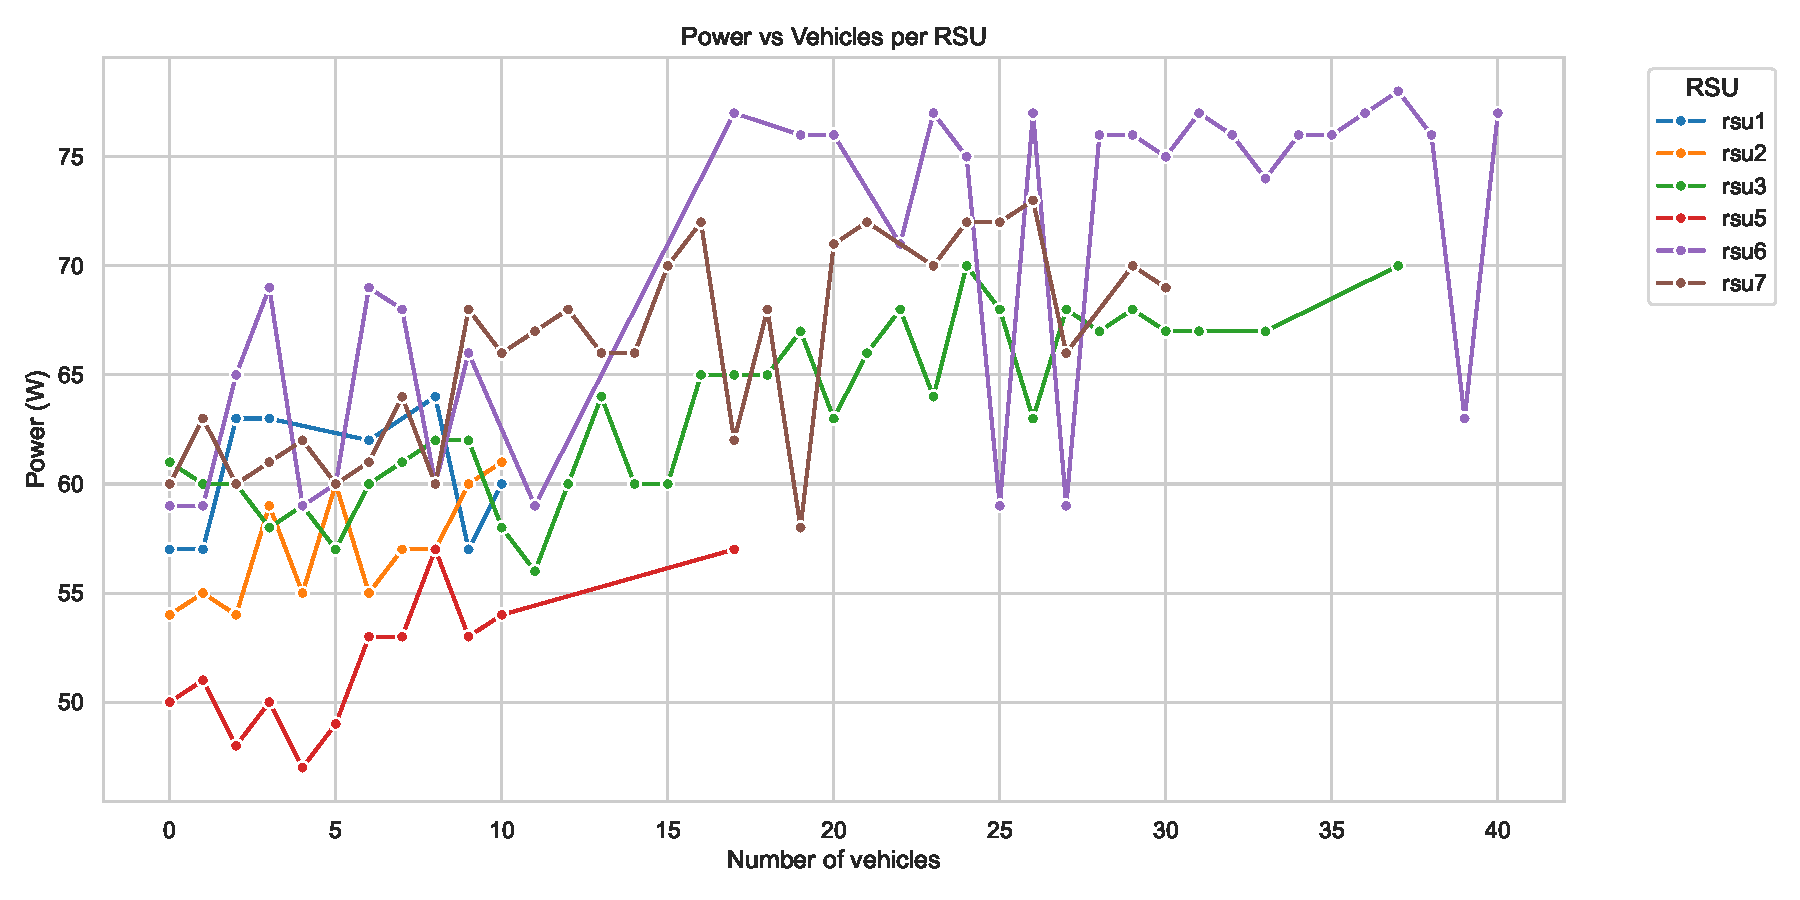
\includegraphics[width=1\columnwidth]{Topics/Energy-Awareness/Figures/power_vehicles_rsu_maximums.pdf}
    \caption{Relationship between the number of vehicles and power consumption for each \gls{rsu}, showing how power usage increases with load and plateaus at maximum capacity.}
    \label{fig:exp1-figure}
\end{figure}